\chapter{HyperSpy quantification}
\label{appendix:HSquant}

The following notebook \dots
% \includepdf[pages=-,pagecommand={},width=\textwidth]{chapters/HyperSpy-quantification.pdf}



\chapter{SE images}
\label{appendix:SE_images}

These are the SE images of the GaAs and GaSb specimen.


%figures/SE_images/Overview_GaAs_GaSb.jpg
\begin{figure}[htbp]
    \centering
    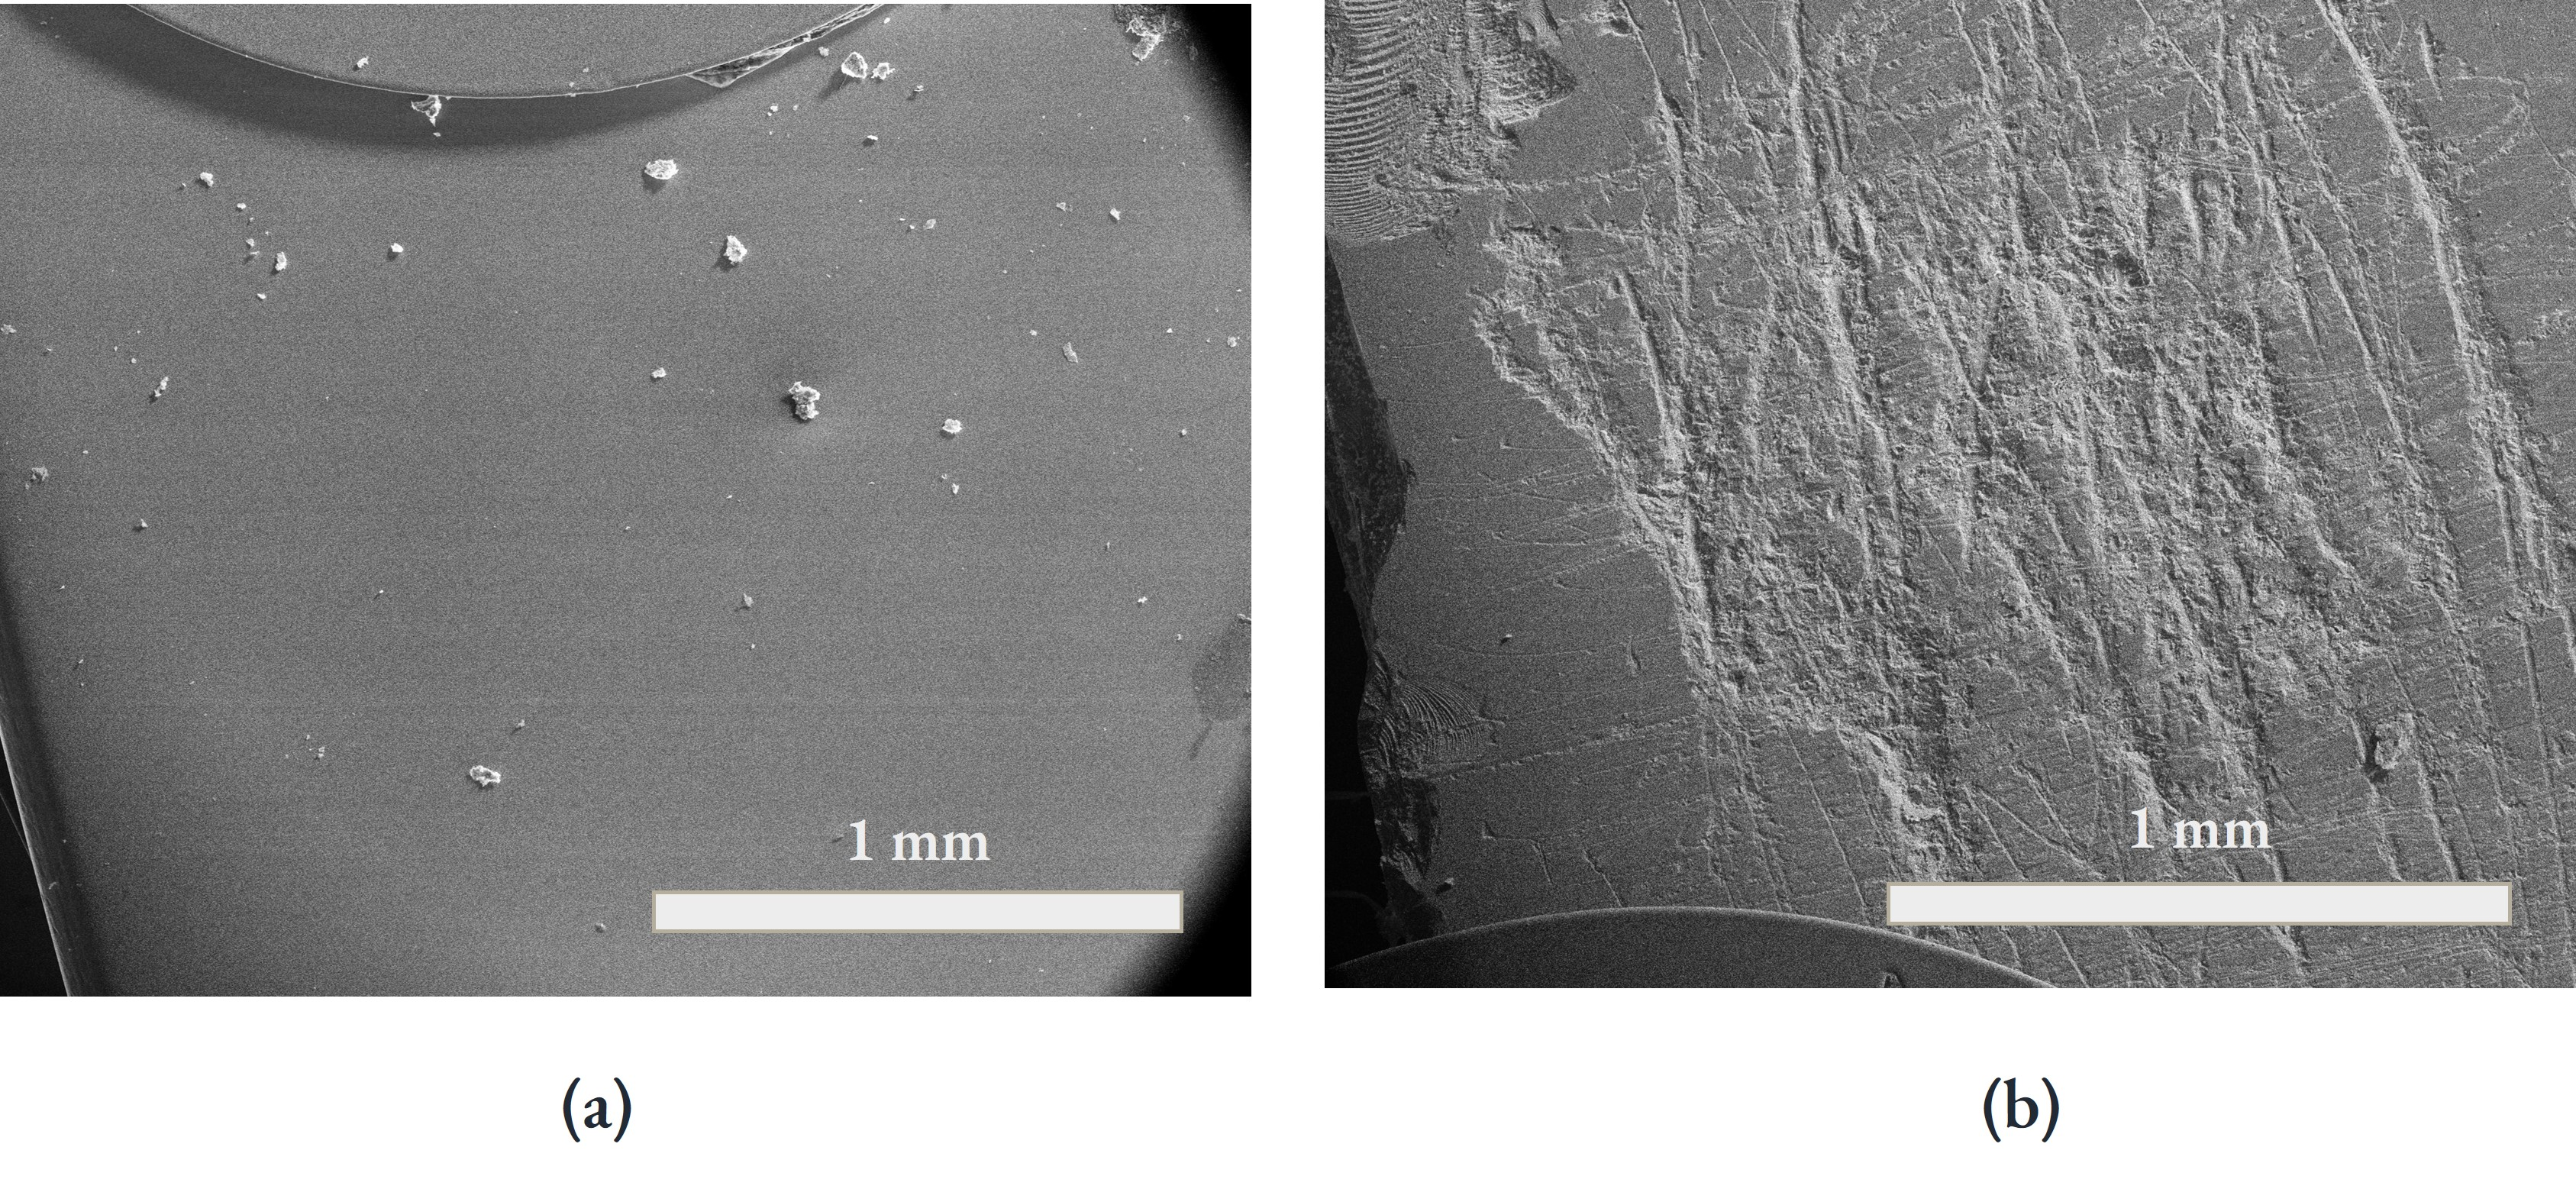
\includegraphics[width=.95\textwidth]{figures/SE_images/Overview_GaAs_GaSb.jpg}
    \caption{
        Overview of the GaAs and GaSb specimen.
        The spectra are acquired in the middle of the images.
        Panel (a) is GaAs, and panel (b) is GaSb.
        The Cu TEM grid is visible at the top and bottom of the images as the large circular object.
        The GaSb wafer have areas which are very scratched, but also areas which are smooth.
        }
    \label{fig:SE_images:Overview_GaAs_GaSb}
\end{figure}

\begin{figure}[htbp]
    \centering
    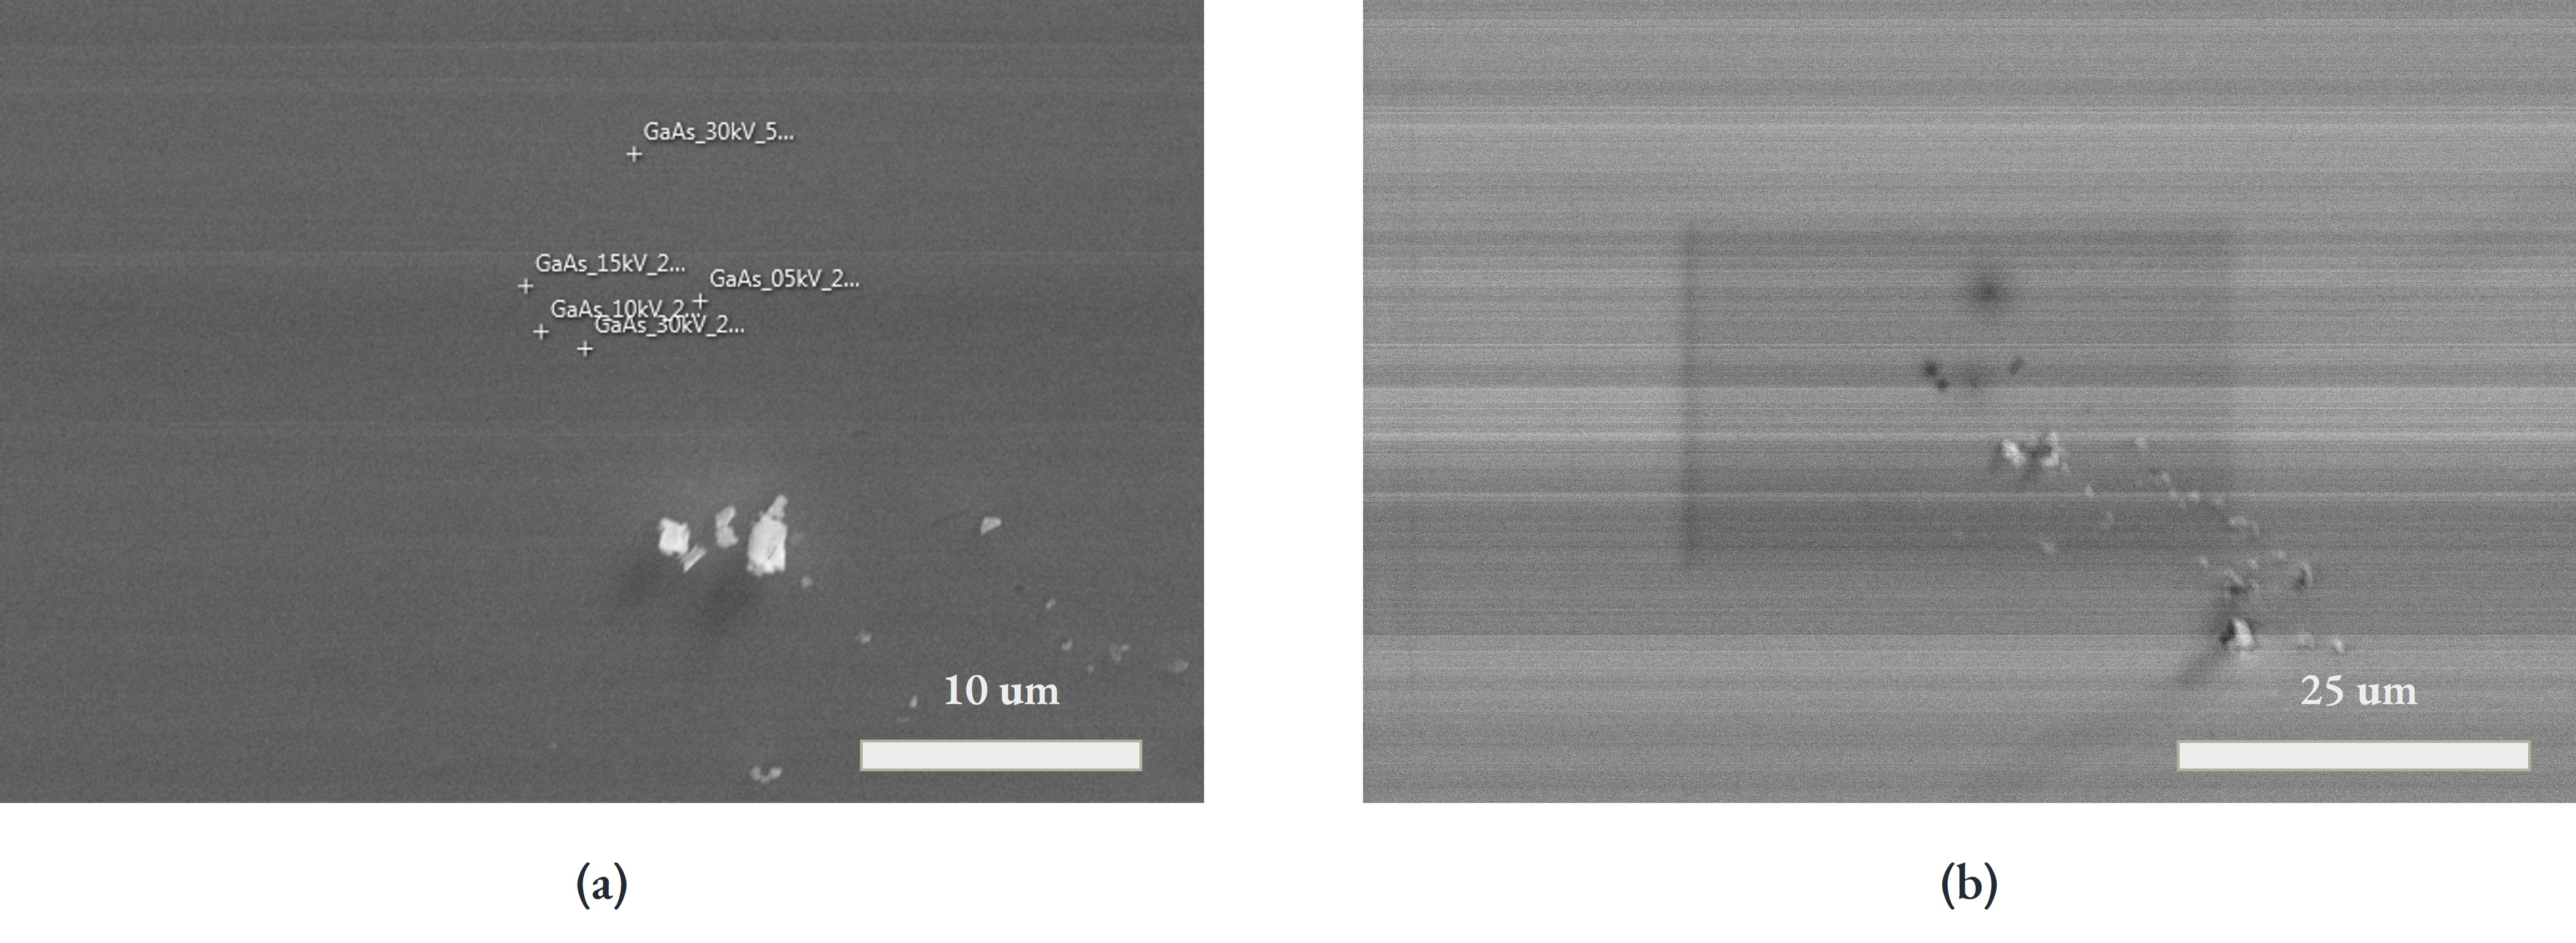
\includegraphics[width=.95\textwidth]{figures/SE_images/GaAs_close.jpg}
    \caption{
        Close up of the GaAs specimen.
        Annotated in panel (a) are the areas which were analyzed.
        Panel (b) is a zoomed out view of the area in panel (a), after the spectra have been acquired.
        This image show both beam damage from the focused probe beam as black dots, and the whole area from the scanning of the probe beam.
        }
    \label{fig:SE_images:GaAs}
\end{figure}


\begin{figure}[htbp]
    \centering
    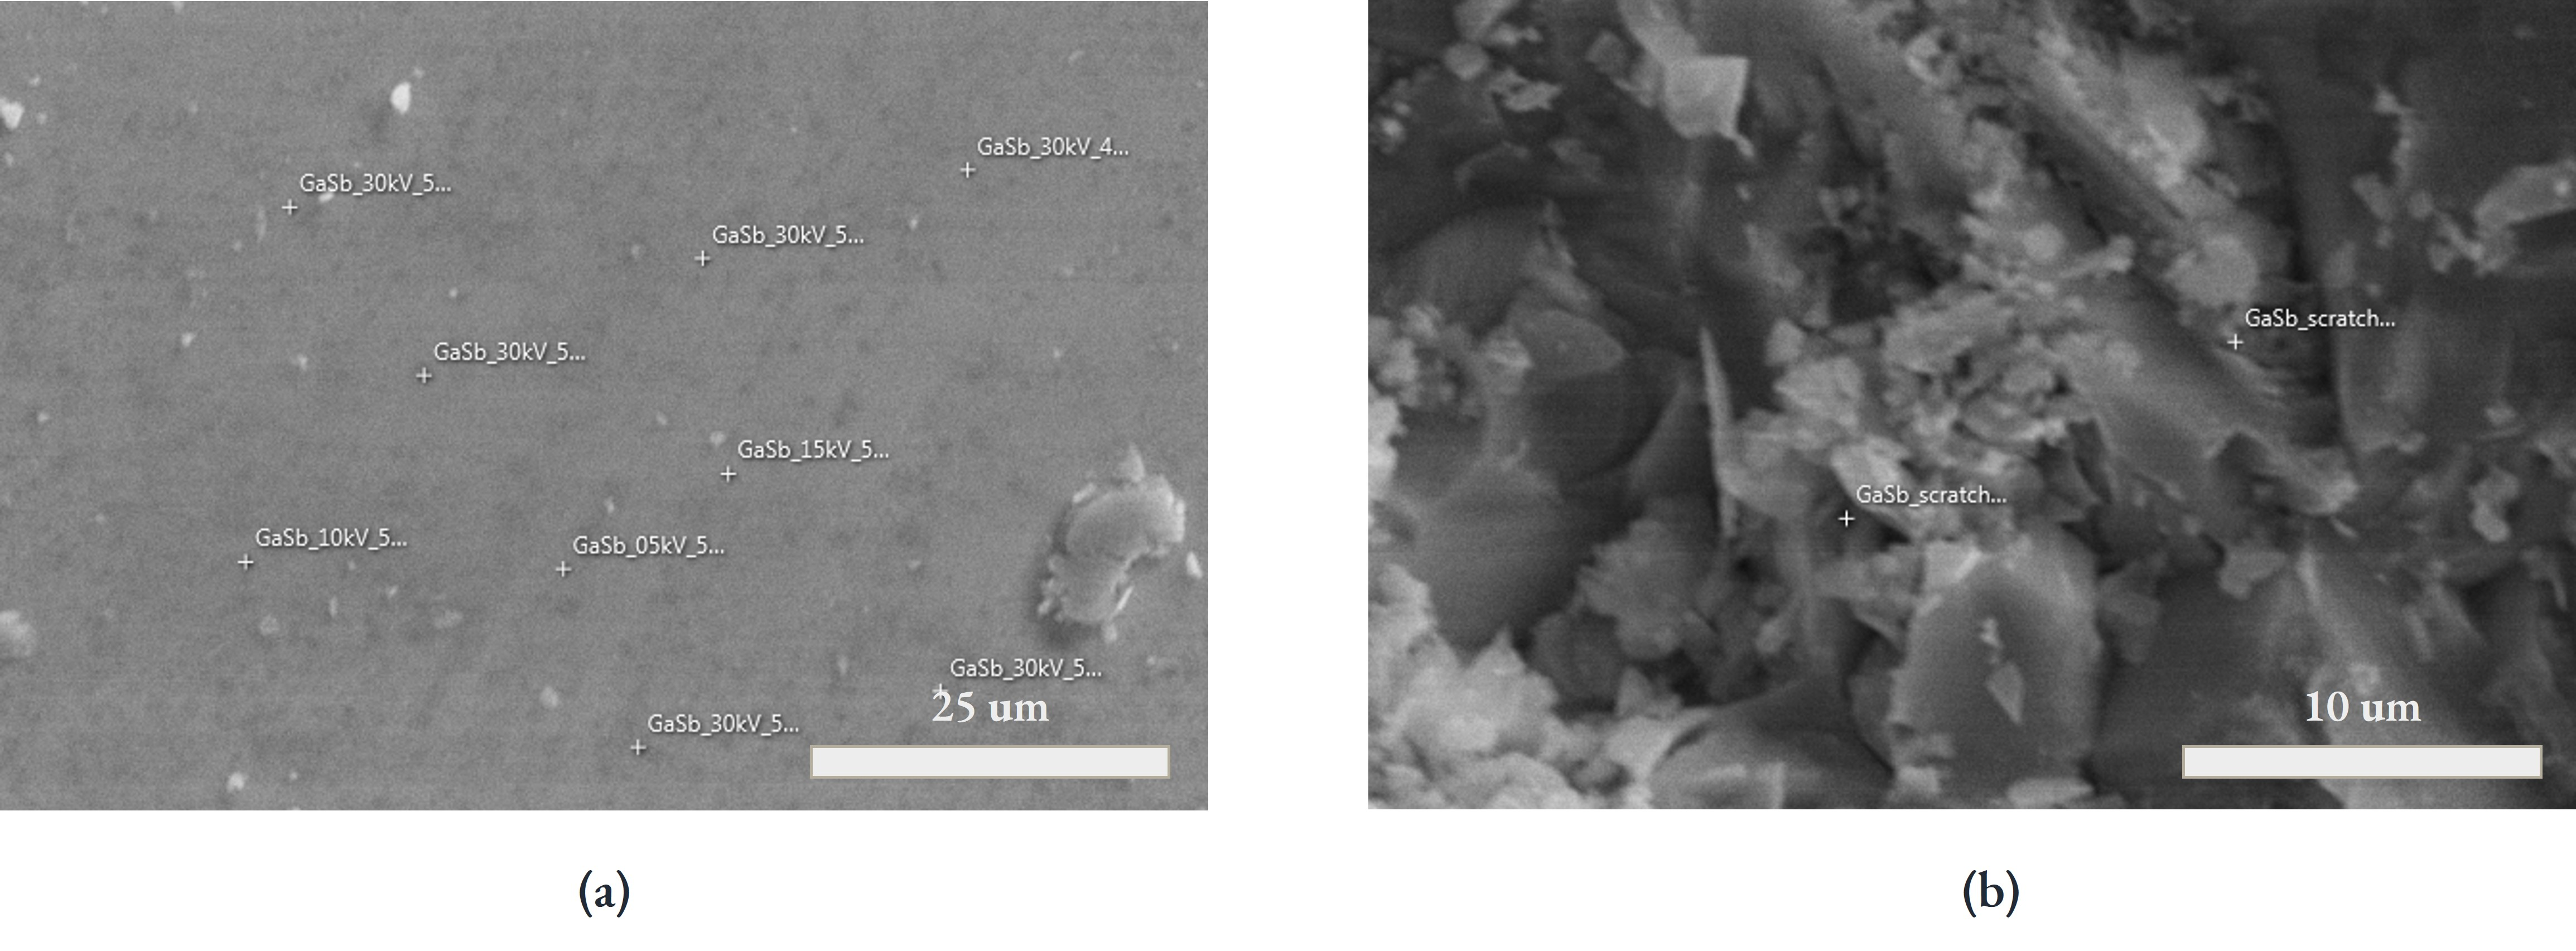
\includegraphics[width=.95\textwidth]{figures/SE_images/GaSb_close.jpg}
    \caption{
        Close up of the GaSb specimen, where the point spectra were acquired.
        Panel (a) is the polished area, and panel (b) is the scratched area.
        Both panels are annotated with the areas which were analyzed.
        }
    \label{fig:SE_images:GaSb}
\end{figure}


\begin{figure}[htbp]
    \centering
    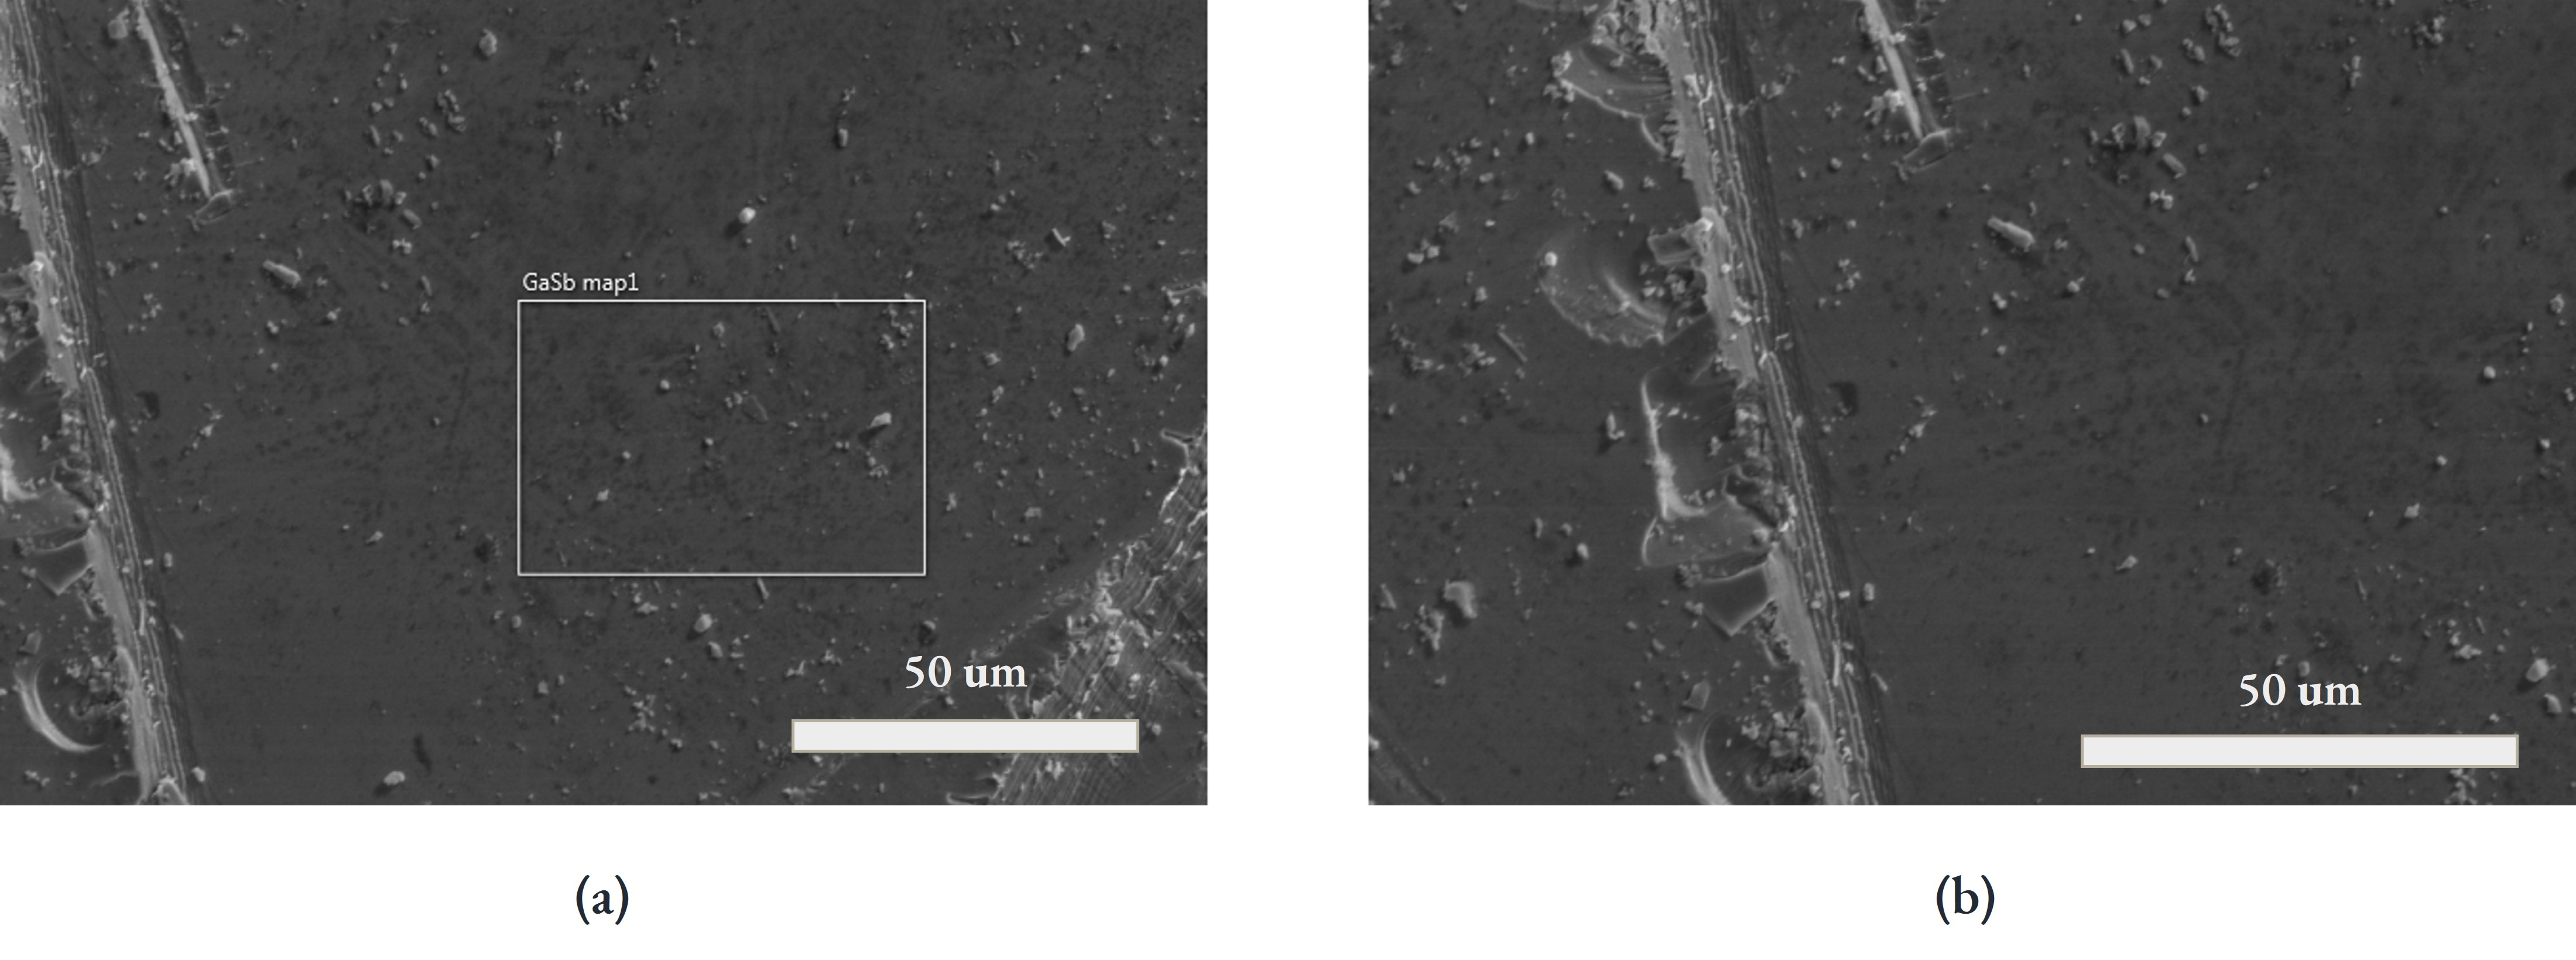
\includegraphics[width=.95\textwidth]{figures/SE_images/GaSb_map.jpg}
    \caption{
        Close up of the GaSb specimen, where the map spectra were acquired.
        Panel (a) is map 1 (within the rectangle), and panel (b) is map 2 (the whole image).
        Map 2 includes one scratched line in the analyzed area.
        }
    \label{fig:SE_images:GaSb_map}
\end{figure}



% \chapter{Plotly plotting}
% \label{appendix:plotting}

% Insert description.

% Insert the code here.